\documentclass[conference]{IEEEtran}
\IEEEoverridecommandlockouts
% The preceding line is only needed to identify funding in the first footnote. If that is unneeded, please comment it out.
\usepackage{cite}
\usepackage{amsmath,amssymb,amsfonts}
\usepackage{algorithmic}
\usepackage{graphicx}
\usepackage{textcomp}
\usepackage{xcolor}
\usepackage[ruled,vlined]{algorithm2e}

\def\BibTeX{{\rm B\kern-.05em{\sc i\kern-.025em b}\kern-.08em
    T\kern-.1667em\lower.7ex\hbox{E}\kern-.125emX}}
\begin{document}


\title{Smart Oracle Based Building Management System }

\author{\IEEEauthorblockN{Angan Mitra}
\IEEEauthorblockA{\textit{Qarnot Computing} \\
Paris, France \\
angan.mitra@qarnot-computing.com}
\and
\IEEEauthorblockN{Yanik Ngoko}
\IEEEauthorblockA{\textit{Qarnot Computing}\\
Paris, France \\
yanik.ngoko@qarnot-computing.com}
\and
\IEEEauthorblockN{Denis Trystram}
\IEEEauthorblockA{\textit{University Grenoble Alpes } \\
Grenoble, France \\
denis.trystram@univ-grenoble-alpes.fr}

}

\maketitle

\begin{abstract}
Buildings in residential and commercial sites consume close to 40 per cent of the world’s total energy produced and is growing at a steady pace. The need to lower the energy footprint is a matter of sustainability and active research for the smart building community. Recent trends in machine learning have led to significant work on occupancy detection in spaces by training isolated or ex-situ models, but with no reliability of performance on unknown spaces. Model applicability becomes questionable when the sensor value distribution is different from training data and in a real-life this is usually the case. Furthermore, analyzing a space on a floor-plan in silo obscures the holistic view of interactivity between building elements. In this paper, we propose the design of a generic building management system that auto-learns occupancy patterns and leverages spatial organization to deliver actionable insights on energy savings. We combine the building information with sensor signals into a Spatio-temporal activity graph, whose edges are dynamically updated based on occupancy. We introduce human-space interaction models to infer the human transmission capacity of each edge and compute an Eigenvalue score for all the spaces to derive automated checkpoints on space-wise appliance monitoring.


\end{abstract}

\begin{IEEEkeywords}
Smart Buildings, Occupancy Prediction, Spatial Energy disintegration, Building Management System, Edge Computing
\end{IEEEkeywords}

\section{Introduction}
\label{section:introduction}
Traditionally speaking a majority of the existing buildings were not designed to cater to automated building intelligence, since a smart building blueprint additionally takes into account optimal sensor placements, network connectivity strength and positioning of mechanical and electrical equipment like fire alarms, power, ventilation, lighting and security systems. Cheap availability of ambient sensors, smart lighting and energy meters has facilitated in an adhoc incorporation of IoT products in buildings. Usually the gain in embedding sensors is leveraged by a Building Management System (BMS), a set of computer controlled processes used to monitor and regulate equipment inside a building. The main objective of a BMS is to derive actionable insights for comfort monitoring, energy management and functional decomposition over a set of spaces. The streaming data accumulated throughout the life span of a building contains sensitive information in the order of Terabytes and a 2019 report~\cite{forecast2019cisco}  by Cisco states that mobile and IoT devices by 2025 will generate close to 850 Zeta Bytes of data which raises significant operating concerns for cloud volumes. Ideally a BMS shall run within premises, compress streaming  data on the fly and most importantly be self-explainable to a non-technical operator or user. The first phase of our work builds a 3D parser to construct an ontology representation from a Building Information Modelling file. The key output of the process is to build a structural information graph where spaces/rooms are the nodes with or without ambient sensors, and edges represent 2D or 3D connectivity via doors, windows or stairs. The second part consists of logic driven oracles that are responsible for auto-tagging sensor data, training of machine learning models and reporting occupied status of spaces. Linking of the two parts enables our proposed system to dynamically react to occupancy changes and focus on likely spaces of  energy footprint. The extracted knowledge can be saved port-ably in a Resource Descriptive Framework (RDF)  or a network graph format like graphml /xml format.


The reminder of the paper is organised as follows. Section \ref{section:relatedwork} introduces the existing state of art in describing buildings and highlights the problem of self-acquiring/updating ambient intelligence. In section \ref{section:spatial}, we introduce a novel representation of building and define a set of geometric objects with algebraic operators to generate a spatial connectivity graph amongst building elements from an ISO standard BIM file. Section \ref{section:ambient} deals with deriving automated insights about occupancy and energy consumption by leveraging the building graph. The proposed methods are evaluated against a test-bed of IFC files and sensor readings from a real-life setting at Paris in Section \ref{section:evaluation}. Finally, conclusions and probable directions for future work are discussed in Section \ref{section:conclusion}.




\section{Related Work}
\label{section:relatedwork}

\begin{figure}[]
\centering
  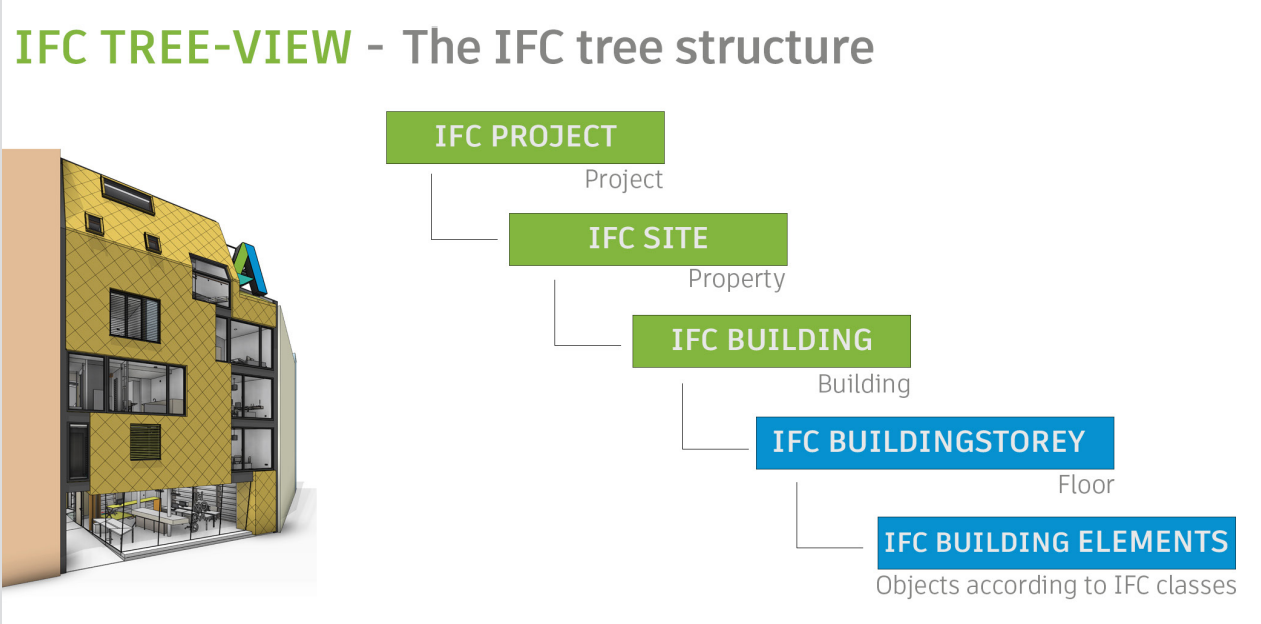
\includegraphics[width=0.7\linewidth]{./img/ifctree.png}
  \caption{Hierarchical arrangement of Industry Foundation Classes objects.}
  \label{fig:ifctree}
\end{figure}


Building Information Modeling (BIM) is the process of designing physical orientations and specifying functional semantics of spaces. Industry Foundation Classes (IFC) is a standard ISO digital format for BIM that is widely popular and is mandatory for European construction projects. But it a complex task to look at an ".ifc" file and answer spatial queries like "Is the bathroom beside the kitchen?", "What is the path to go from point A to B?". Authors of BRICK \cite{balaji2018brick} state the bottleneck as IFC being largely oriented for designing and construction of buildings. As shown in Fig. ~\ref{fig:ifctree}, IFC is an entity-relationship model with several thousand entities organized as in a referential structure.  The root of an IFC Project defines an arbitrary origin (IfcSite) with an optional mapping to physical coordinates of a real building. As per IFC standards, a building is organized into storeys (IfcStorey) or floors. Typically a storey consists of building elements like walls, doors, windows, spaces, stairs etc. Each element has a set of properties (IfcObjectProperty) that define material type and spatial orientation. The starting coordinates (0,0,0) of any building element is given as an offset with respect to its parent's origin and geometry is defined in its Local Coordinate System. A locally defined point of a building element needs to be 3D translated recursively in a bottom up manner all the way up to IfcSite to get the real world coordinates. Such referential geometry is extremely useful during an incremental construction process but comes with a high computation load. The existing literature lacks clarity of how one can derive geometric ontology from an IFC file.  

Building Management System (BMS) \cite{liu2021indoor} is a set of computer-controlled processes that monitor and act on building health and security. The initial interest for developing BMS was automated control with lower energy foot-printing. The authors \cite{bazjanac1999industry} give a proof of concept on  energy savings through automatic exchange of building geometry for building design processes. A related work ~\cite{bhattacharya2016enabling} extracts a sensor's placement information from an IFC file and constructs a query based metadata structure to find faulty Air Handling Units in Heating Ventilation Air Conditioning systems. The utility of building metadata becomes evident when it is enriched \cite{roth2014open} \cite{balaji2018brick} with sensor readings to derive causal relations amongst spaces ~\cite{cook2003mavhome} and define signature activities \cite{stavropoulos2012bonsai}. The aim is to decompose ~\cite{cook2003mavhome} a temporal stream of sensor data coming from multiple spaces into cause and effect clauses. ~\cite{cumin2017human} enlists possible activities in commonly known spaces and associates a classifier per situation for place-specific activity recognition in a closed world setting. There are a variety of smart building applications like occupancy detection ~\cite{garg2000smart}, ~\cite{ai2014occupancy}, anomaly detection \cite{capozzoli2018automated}, energy saving \cite{mitra2016economical}, \cite{ostadijafari2020linearized}, air quality monitoring \cite{dong2019review}, activity detection ~\cite{dong2009sensor} etc. Existing research in smart buildings focus on designing ex-situ algorithms but provide no or limited insight on explainable nature or auto-update scheme of models or data retention policy at deployment site etc. Different spaces can generate non-identical patterns on identical sensors. For example in a room with window there is a gradual increase in luminosity values from dawn till mid day before decreasing to 0 at night, but in a window-less room we see a sharp rise and fall in sensor values when lights are on and off respectively as shown in Figure \ref{fig:luxComparison}. Table \ref{table:datadistribution} enlists some explanations to highlight peculiarities in smart building data across heterogeneous spaces. Furthermore, authors \cite{mitra2021impact} shows the effectiveness of in-situ machine learning for a smart building by performing in-house federated learning for forecasting sensor values. This forms the motivation for our edge application which forms a digital twin of a building and applies artificial intelligence for meaningful insights. 


\begin{table}[]
\caption{Possibility of sensor distribution variation due to spatial and usage constraints }
\label{table:datadistribution}
\begin{tabular}{|l|l|l|}
\hline
Sensors     & Observations    & Reason                                                                         \\ \hline
Light       & Bias            & Placed in a space with window \\
&   &   and there is ample sunlight.                     \\ \hline
Light       & Activity signal & Placed in a space without window \\
&   &    and is switched on during an activity.     \\ \hline
Temperature & Bias            & Sensor placed close to probable heated \\
&   &   surfaces or has strong incident light. \\ \hline
Sound       & Activity Signal & Placed in a room where human \\
&   &   activity generates sound.                         \\ \hline
Sound       & Bias            & Placed in a noisy environment. \\ \hline
Motion      & Bias            & Placed incorrectly so that it \\
&   &   gets unwanted signals.                           \\ \hline
Motion      & Activity Signal & Placed in a space to detect \\
&   &    if the space has human intervention.               \\ \hline
\end{tabular}
\end{table}

\begin{figure}
\centering
  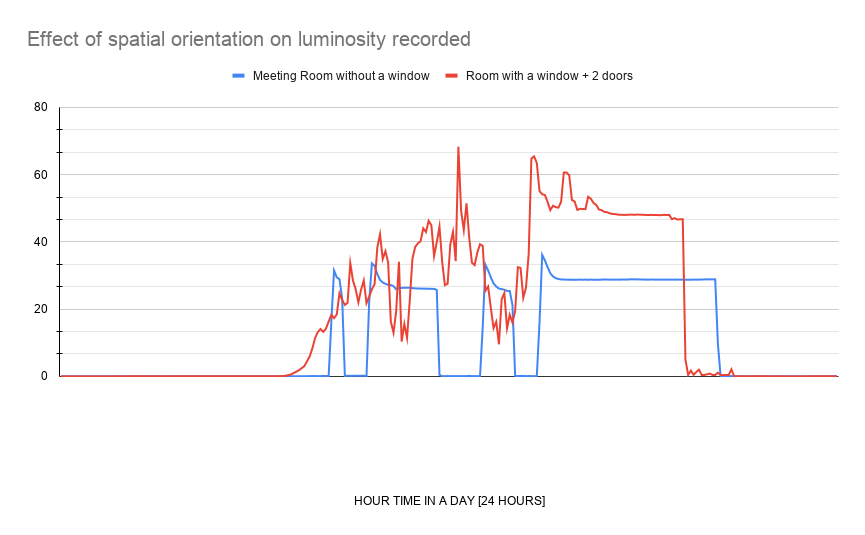
\includegraphics[width=1\linewidth]{./img/luxDayComparison.png}
  \caption{ Luminous variation between rooms with and without windows in red and blue respectively.}
  \label{fig:luxComparison}
\end{figure}


 



\section{Spatial Intelligence }
\label{section:spatial}

The complexity of an IFC file grows with increasing number of IFCProducts like spaces, doors, windows, stairs, roofs, stories etc. or intricacy in level of detailing. It is non-trivial to open an IFC file in a text editor and guess the link between a door attached to a space. For querying relationships amongst building elements, IFC proposed a Resource Description Framework to represent building in Ontology Web Language, namely IFC OWL. The referential coordinates of a building product are kept unchanged in such a translation and this complicates geometrical reasoning about adjacent or overlapping building elements. Also from the software perspective, there is lack of an open source parser, that can directly generate a per storey floor-plan from IFC file of a building.
We introduce two geometric objects: a bounding box and a 3D plane that operates on referential geometry of an IFC object and outputs element coordinates in a single-origin reference frame defined on IFCSite. 


\textbf{Building Box $\mathcal{B}$} is a rectangular parallelepiped enclosing a building element and represented by a pair of coordinates per axis. Each axis pair contains the maximum and minimum coordinates enclosing the box along that axis. Formally we will represent the \textbf{Building Box} Representation of a building element $\mathcal{E}$ as 
\begin{equation}
  \begin{aligned}
  \mathcal{B}_X(\mathcal{E}) &= \{ X^{Min}(\mathcal{E}) ,  X^{Max}(\mathcal{E})   \} \\
  \mathcal{B}_Y(\mathcal{E}) &= \{ Y^{Min}(\mathcal{E}) ,  Y^{Max}(\mathcal{E})   \} \\
  \mathcal{B}_Z(\mathcal{E}) &= \{ Z^{Min}(\mathcal{E}) ,  Z^{Max}(\mathcal{E})   \} \\
      \end{aligned}
\end{equation}

\textbf{Cutting Plane $\Xi$} is an imaginary plane that passes through a building and is defined by Equation \ref{eq:cutting-plane} where $\hat{n}$ and $\vec{P_0}$ represents the normal vector and a fixed point on the plane. $\vec{P_0} = (0,0,z)$, $\vec{n}=(0,0,1)$ denotes the family of horizontal planes placed at height \textit{z} from the ground plane. 

\begin{equation}
    \Xi (\vec{P}_0, \hat{n}) \equiv \hat{n}(\vec{p}-\vec{P_0})=0
    \label{eq:cutting-plane}
\end{equation}

\subsection{Parsing Algebra}
We demonstrate an algorithm that gives a controllable process to generate a floor-plan from one or more cutting planes and infer a connectivity graph amongst building elements. In the process, we develop useful operators to algebraically formulate building aware intelligence use-cases like neighbourhood, path and ventilation graph. 


\subsubsection{Selection}
 The system generates the 3D view of all IFC Products with defined shapes and stores the Bounding Box representation in 3 interval trees, one for each axis. Each node contains the minimum and maximum points along one of the axes.  $p$ building elements or intervals can be arranged in an interval tree ~\cite{de1997computational} as shown in Fig.~\ref{fig:intervaltree}. Such trees have an initial creation time of $O(p \log p)$ and output sensitive query time of $O(\log p + m)$ depending on number of matches $m$.  The memory consumption is limited to $O(p)$.
$\sigma$ : $\{$\textbf{Building Element} $\}$ $\times$ \textbf{Query Point} $\rightarrow \{$ \textbf{Building Element}$ \}$  returns the set of building elements $B$ whose bounding box encloses the point from all 3 axes.  
\begin{equation}
    \sigma(B, (p,q,r)) = \{ \mathcal{E}|\mathcal{E} \in B ,  p \in \mathcal{B}_z(\mathcal{E}) , q \in \mathcal{B}_z(\mathcal{E}) ,  r \in \mathcal{B}_z(\mathcal{E}) \}
    \label{eq:select}
\end{equation}


\begin{figure}[]
\centering
  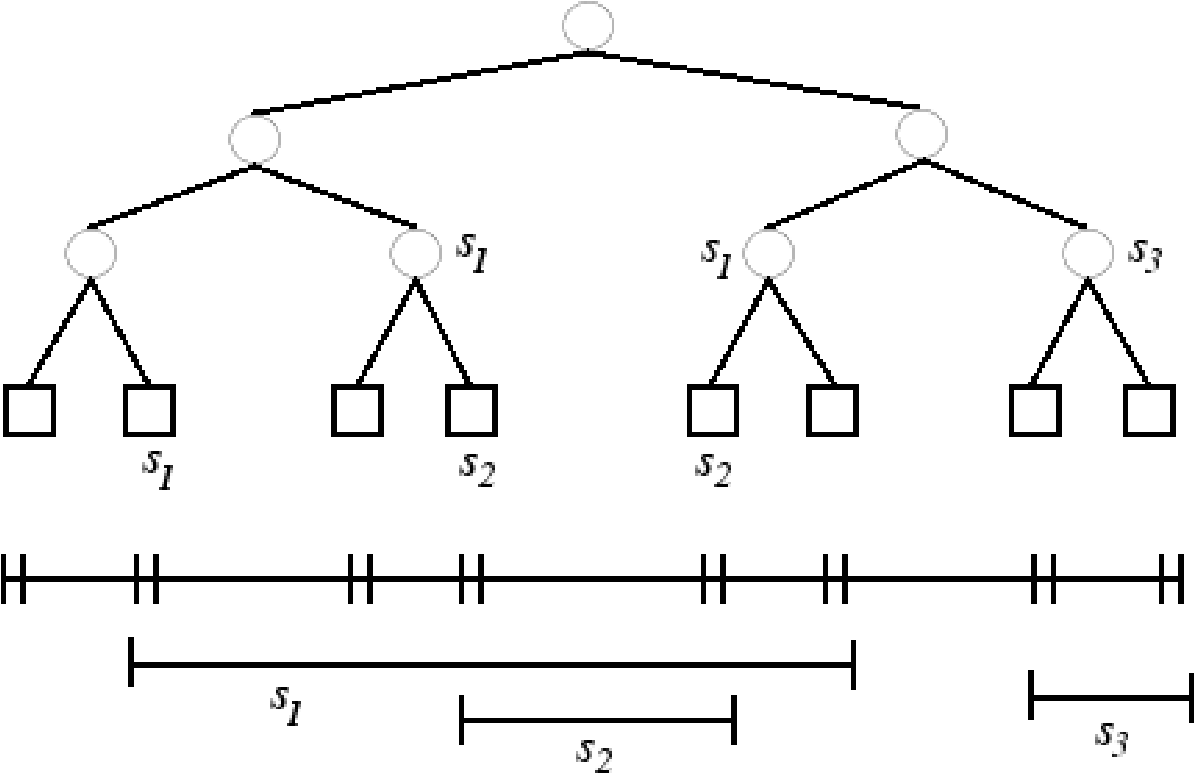
\includegraphics[width=0.5\linewidth]{img/intervaltree.png}
  \caption{Illustration of an interval tree, intervals denoted by $S_1, S_2 \& S_3$   }
  \label{fig:intervaltree}
\end{figure}



\subsubsection{Contour}

{Element Contour $\mathcal{C}$} : $\{$\textbf{Building Element} $\}$ $\times$ \textbf{Plane} $\rightarrow \{$ \textbf{2D Points}$ \}$ returns a set of intersection points that are generated by the impression of a building element on a cutting plane. The smallest convex set of points that contains the element is the contour or hull of impression. We define Element Contour of a building element $\mathcal{E}$ as an ordered set of intersecting points given by Equation \ref{eq:contour}. For a building object located above or below a plane $\mathcal{C}(\mathcal{E}, \Xi) = \phi$ since there are no intersecting points.
\begin{equation}
    \mathcal{C}(\mathcal{E}, \Xi) = \{ (u_i,u_{i+1}) \} | \forall i \in [1,2,\dots, p],  u_{p+1}=u_0
    \label{eq:contour}
\end{equation}



\subsubsection{Hull }

The next task is generating a singular impression of a building object from multiple element contours. We recall the well studied concept \textbf{Delaunay Triangulation} ($\mathbf{DT}$) of a set of triangles constructed from a set(P) of planar points such that no point in P is inside the circumcircle of any triangle in DT. The nominal work~\cite{shamos1976geometric} of sweep line algorithm computes Delaunay triangulation in $O(n\log n)$ expected time with $O(n)$ storage for a polygon of $n$ points.  $\mathcal{H}$ : $\{$\textbf{Element Contours} $\}$ $\rightarrow \{$ \textbf{Element Contour}$ \}$ (Equation \ref{eq:hull}) outputs a mapping for every input data point such that the corresponding coefficient ($\beta_i = 1$) if the point lies on the Delaunay hull or 0 otherwise. A sample of Delaunay triangulation for a door is shown in Fig.~\ref{fig:triangulation}.



\begin{equation}
\mathcal{H}(\{\mathcal{C}\}) = \{  \beta_i \times p_i | \beta_i \in \{0,1\} \forall {i \in\{C\}}  \}
\label{eq:hull}
\end{equation} 

% \begin{equation}
% \mathcal{H}(\{\mathcal{C}\}) = \{ \overline{t} | t \in \mathbf{DT}( \{\mathcal{C}\} ) , \overline {t}\in \mathbf{R}^2  \}
% \end{equation} 

\begin{figure}[]
\centering
  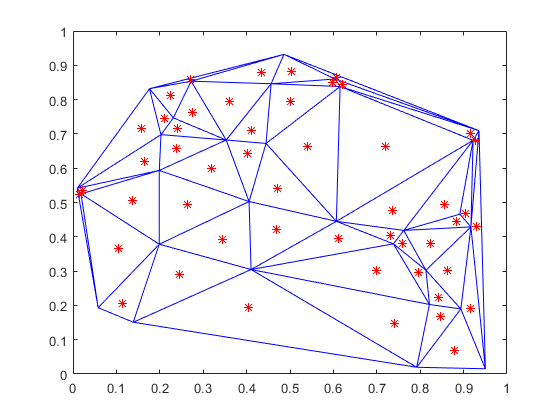
\includegraphics[width=0.5\linewidth]{img/triangulation.png}
  \caption{Hull Generation of a door from multiple contour points (in red) by Delaunay Triangles (in blue) }
  \label{fig:triangulation}
\end{figure}


\subsubsection{Overlap}

{$\Omega$} : $\{\mathcal{C}_1, \mathcal{C}_2 \}$  $\rightarrow \{$ \textbf{0,1}$ \}$  takes two polygons as inputs and if they intersect or overlap the expression evaluates to True or 1. This operator is useful in inferring spatial connectivity between adjacent building elements. One can tweak the connectivity by inflating a hull to make sure the desirable overlap is reached.


For floor-plan generation of a storey, the system generates slicing planes at every $\Delta h = 0.5$ meter and processes multiple contours for every building element to output a convex hull. Multiple hulls on a 2D plane yields a floor-plan. The parsing is controlled by specifying the starting and ending height for cutting plane and fine tune the multiple contour process by tuning the vertical resolution. The parser is written in pure python, supports IFC 2x3, and 4.1 formats and is made publicly available in Docker hub under the image name "angmit/ifcparser:v2.0".


\subsection{Spatial Graph}

We construct a spatial graph ($G^S$) to capture the connection between building elements such as spaces, doors, windows, stairs, elevators, storeys and roof. Nodes (V) of the spatial graph represent elements of interest and a edge between two elements are drawn in case of spatial overlap or intersection. Formally Equation \ref{eq:space-graph} expresses the connectivity graph amongst a set of building elements \textbf{B} through a set of cutting planes $\Xi$. Graph data can be port-ably stored in either a JSON, XML or RDF format which is queried to answer the spatial intelligence use-cases demonstrated below. Each node additionally stores the corresponding IFC identifier and type of element.
\begin{equation}
G^S (V,E)= \{ (u, v) |\forall u,v \in V, \Omega( \mathcal{H} ( C(u, \Xi)),  \mathcal{H} (C(v,\Xi) ) =1\}
\label{eq:space-graph}
\end{equation}


\subsubsection{Neighbours   }

Neighbour discovery is now made possible through geometric reasoning. Queries like "Are there stairs beside the kitchen?" computationally retrieves the list of neighbouring elements for the query building element \textit{kitchen}. We extend the notion of adjacency to \textit{d} hops by exploring nodes in a depth first traversal up-till \textit{d} links from the query node. This is often useful for estimating 1-hop connections between two spaces who share a common door or window. If $N_0(u, w)$ represents a adjacent neighbour (\textit{w}) of an element (\textit{u}), then one hop neighbour graph is given by Equation \ref{eq:one-hop}.
\begin{equation}
G^1(V, E) = \{(u, v) | \exists w, N_0(u, w), N_0(w, v) \}
\label{eq:one-hop}
\end{equation}

\subsubsection{Structural Path }
A path in a building is defined in terms of an ordered set of building elements that can be physically visited while going from space A to B. Logically this means, the path can not pass through a wall or a window or a roof. Equation \ref{eq:path-graph} defines a path graph ($G^P$) of space-space linkages that is constructed  by discarding all edges from $(G^1 \cup G^S)$ whose source or destination is not a space.
\begin{equation}
G^P = \{ (u,v)| (u,v) \in G^S \cup G^1,  u.type \& v.type = space  \}
\label{eq:path-graph}
\end{equation}
A space link is represented by the centroid of a building element ($\vec{\mathcal{E}_i}$) and a displacement vector ($\vec{d}s_i$) connecting the next traversed element. A path ($\mathcal{P}$) starting from building element $\mathcal{E}_p$ and ending at $\mathcal{E}_q$ is an ordered sequence of \textit{L} space links as per Equation \ref{eq:path} . Imposing constraints on linkages can yield a variety of paths. For example, the shortest path with net minimum displacement is specified as $\arg \min_{\vec{d}s}\Sigma_{i \in \mathcal{P}} |\vec{d}s_i|$. A path can also be derived by minimizing number of building elements traversed from by imposing the constraint $ \arg \min_{\mathcal{P} \in P}|  \mathcal{P} (\mathcal{E}_p, \mathcal{E}_q)|$. 

\begin{equation} 
 \mathcal{P}(\mathcal{E}_p, \mathcal{E}_q)  =  \{(\mathcal{E}_{i}, \vec{\delta}s_i)|\vec{\mathcal{E}}_{i+1} = \vec{ \mathcal{E}}_{t} + \vec{\delta} s_i ,
 \& E_0 = \vec{\mathcal{E}_p}, E_L = \vec{\mathcal{E}_q}   \} 
 \label{eq:path}
\end{equation}

\subsubsection{Ventilation View}

$G^B $ can be manipulated to expose views necessary for a building management operator to suit different functional requirements. CO$_2$ build up and dissipation is an important use-case for smart buildings, for which we explicit the construction of ventilation view. We start by pruning edges of $(G^1 \cup G^S)$ where any endpoint does not belong to the IFC elements of interest namely doors, windows, spaces, stairs and elevators. Having such a structural analysis leads to identifying poor ventilated spaces, for example, a room without a window but only a door.  We show the 2D and 3D Circulation views of a building in  Fig \ref{fig:circulationView} and Fig.\ref{fig:3dtraversal} respectively.   Additionally, wall-wall and wall-space contacts are shown in Fig.  \ref{fig:wallSpace} and are generated by retaining edges of $(G^1 \cup G^S)$ where the source or destination element is a wall or space.


\begin{figure}
\centering
  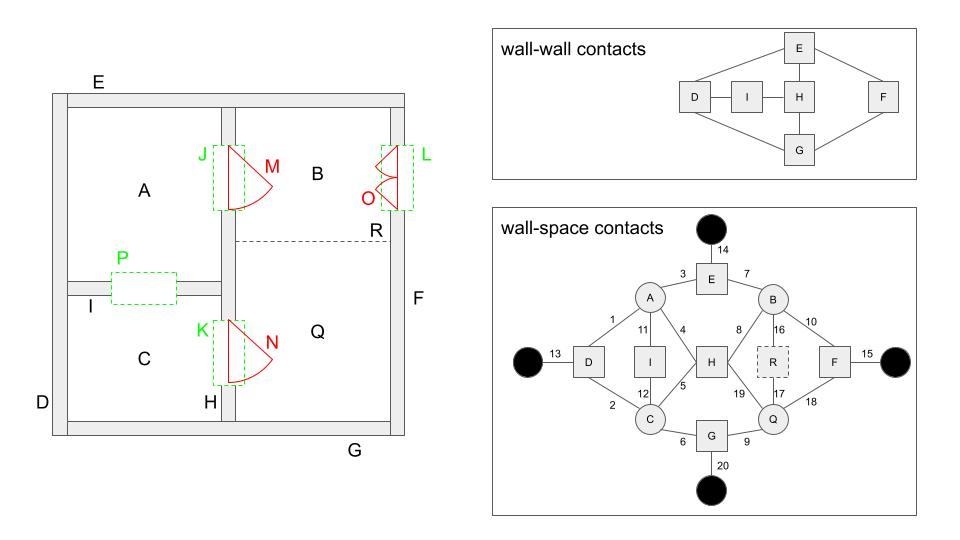
\includegraphics[width=0.99\linewidth]{./img/wallSpace.jpg}
  \caption{ Wall to wall contact and wall space contact graph view from a 2D floor plan. }
  \label{fig:wallSpace}
\end{figure}


\begin{figure}
\centering
  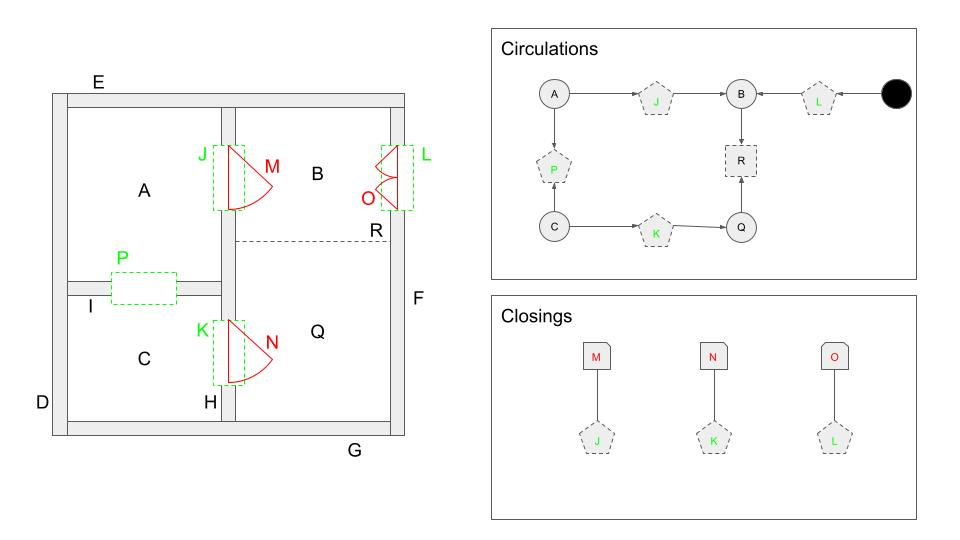
\includegraphics[width=0.99\linewidth]{./img/circulationView.jpg}
  \caption{  Ventilation View abstraction from a 2D floor-plan.  }
  \label{fig:circulationView}
\end{figure}

\begin{figure}
\centering
  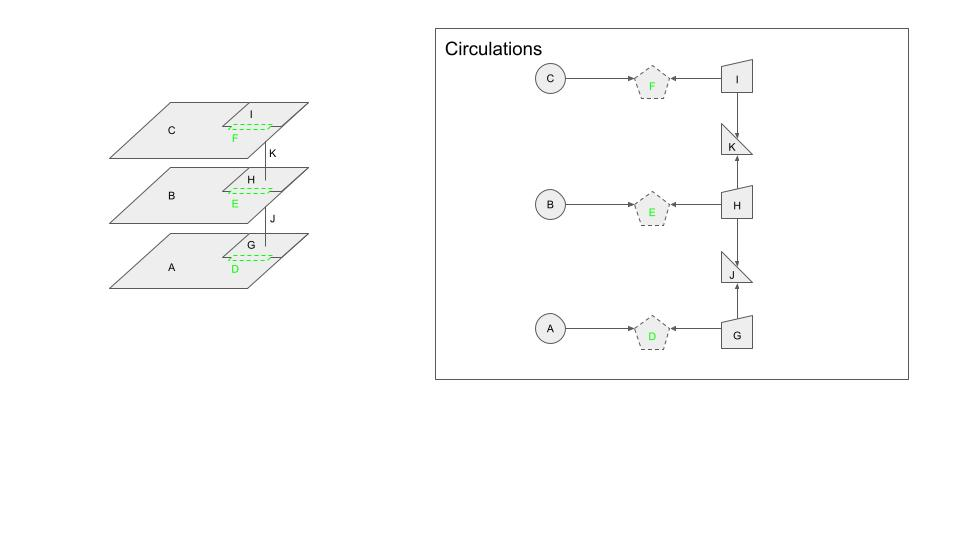
\includegraphics[width=0.99\linewidth]{./img/3dtraversal.jpg}
  \caption{ 3D Movement Capture inside the Spatial Knowledge graph, where K, J represents stairs connected to spaces I,G,H with doors F,E,D leading to spaces A,B,C. }
  \label{fig:3dtraversal}
\end{figure}





\section{Ambient Intelligence}
\label{section:ambient}

\begin{figure}
\centering
  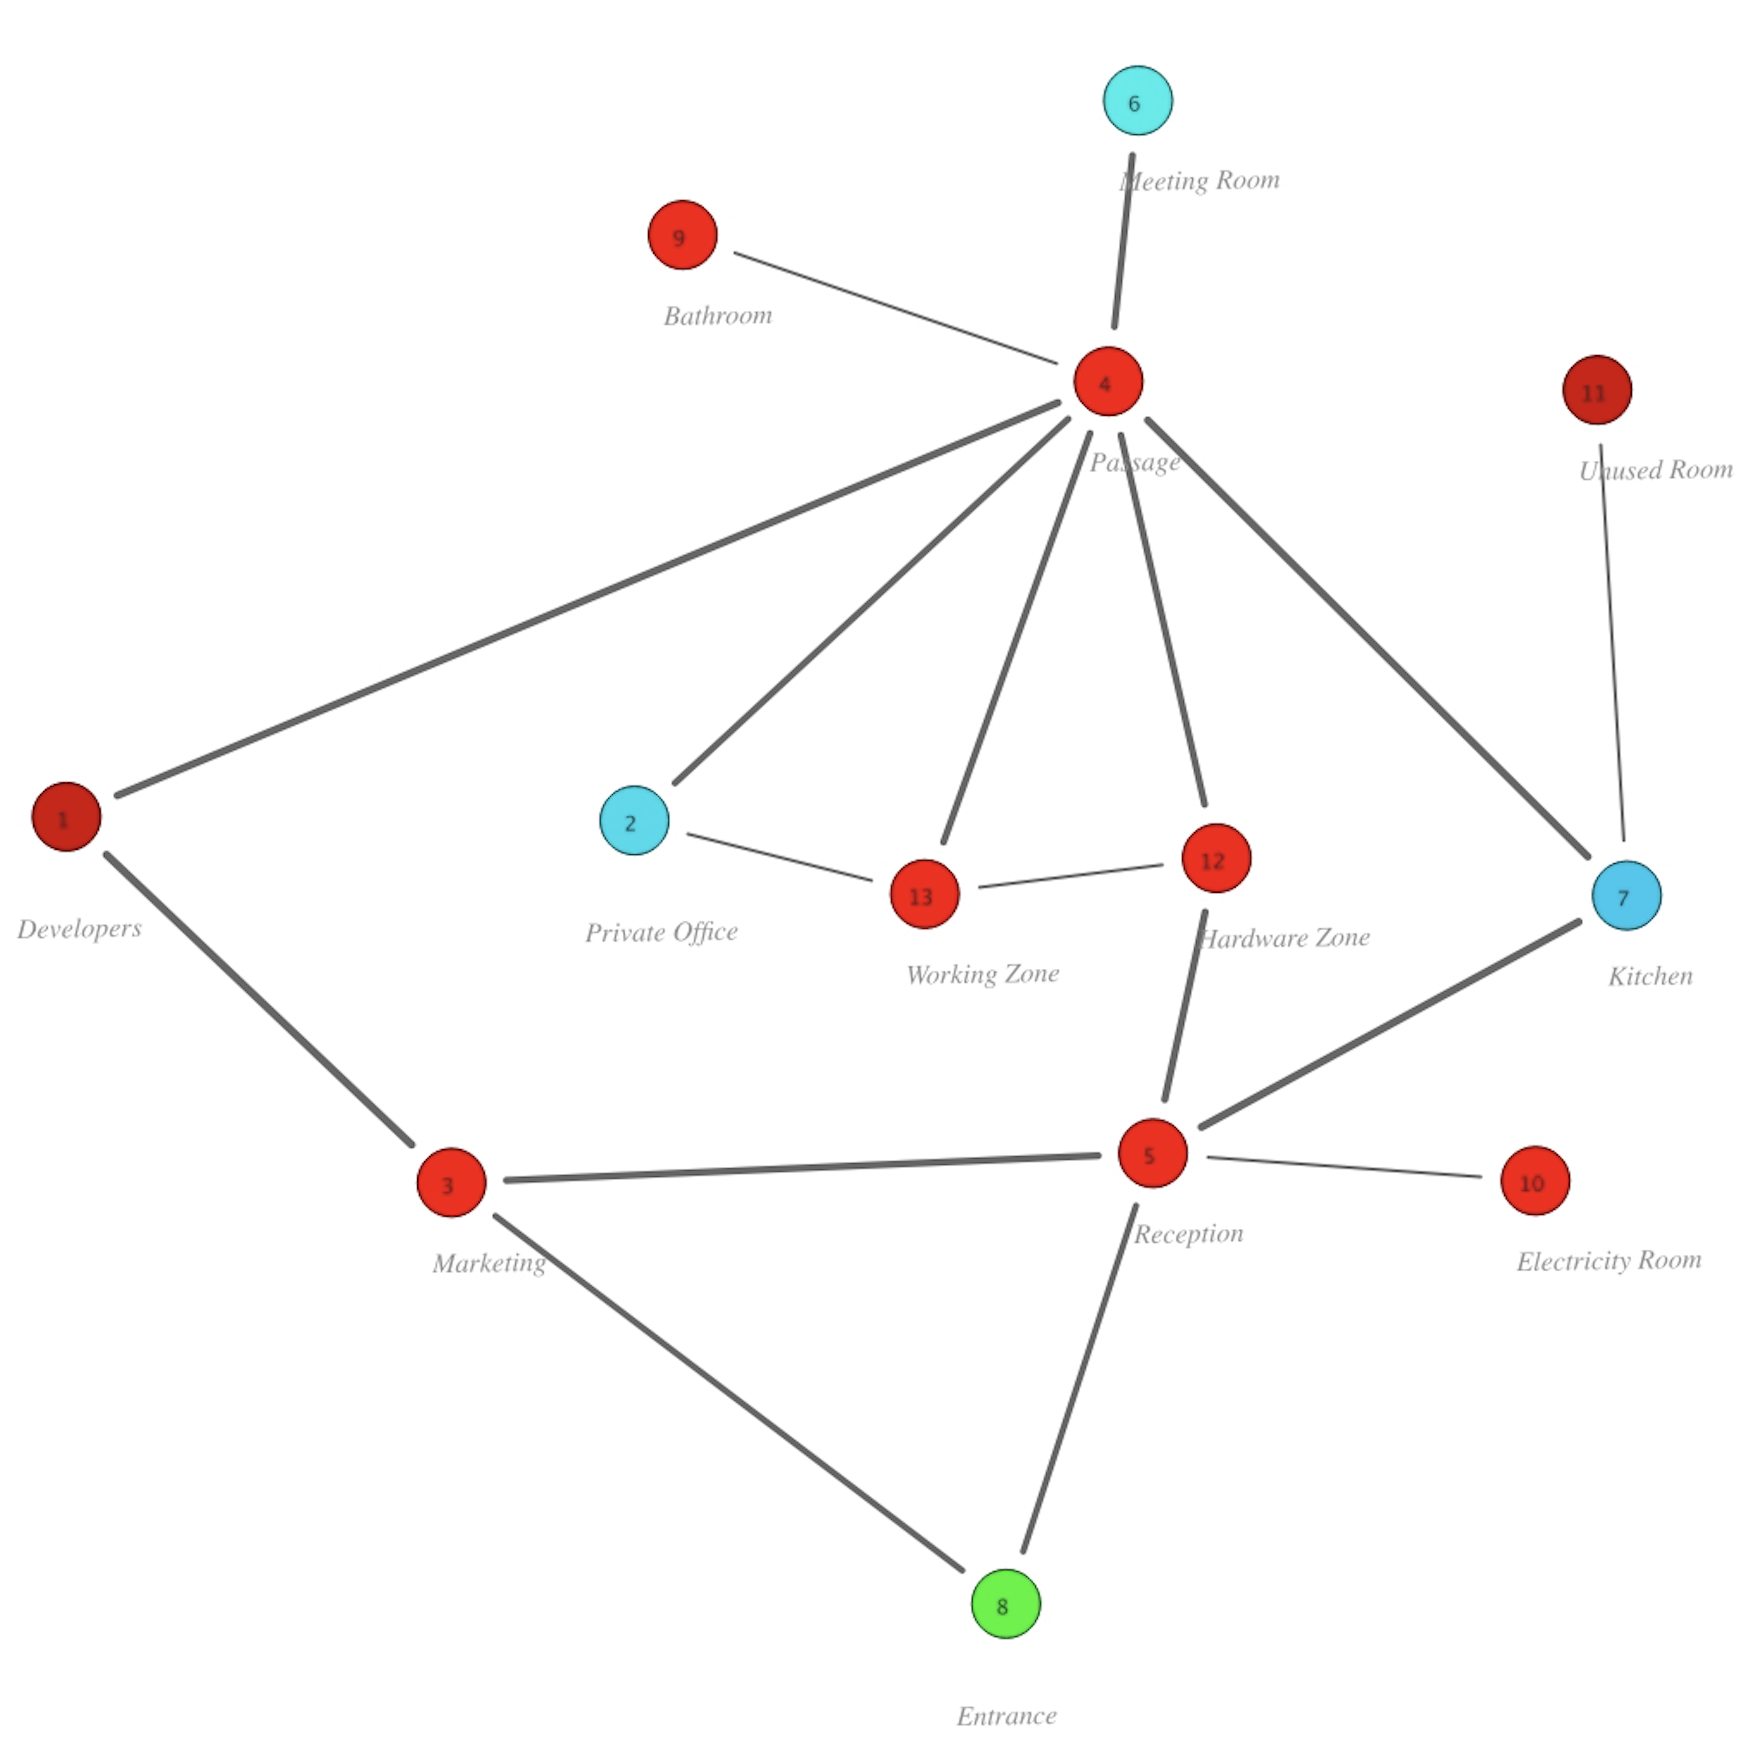
\includegraphics[width=1\linewidth]{./img/energygraph.png}
  \caption{ Spatial Path Graph ($G^P$) of spaces in the floor-plan. The points in blue are spaces where sensors are placed and access to the floor-plan is highlighted in green. }
  \label{fig:energygraph}
\end{figure}


We introduce a use-case of energy monitoring that leverages activity detection with spatial graph to derive automatic energy savings insights. The motivation is to detect chronologically active spaces and extract semantically rich or most utilised paths. For example, the paths that lead towards entering or exiting a floor-plan is likely to be most utilized during office beginning or ending hours respectively. Similarly at noon, employees are usually expected to leave their working spaces and gather at the kitchen/cafeteria for lunch. After an activity happening at space $S_0$ comes to an end, people will disperse from that location and is likely to traverse/occupy adjacent spaces. We label the power consumed as wasted when there is no occupancy and non-essential appliances like desktop monitors, laptop chargers, printers etc. are running. $WE(s, t) =  (1-O_s^t) \times P^t_s$ gives estimate of waste power where $P^t$ represents the instantaneous power consumed and $O^t \in \{0,1\}$ reflects an empty or occupied space respectively.


We implement the following two stepped process to give an occupancy derived energy score to a space.  

\begin{equation}
    \mathcal{I}^t(V_i,V_j) = max( c_i  \times O_i^t, c_j  \times O_j^t  )
    \label{eq:maxdispersion}
\end{equation}

\begin{equation}
    \mathcal{I}^t(V_i,V_j) = min( c_i  \times O_i^t, c_j  \times O_j^t  )
    \label{eq:mindispersion}
\end{equation}

\begin{enumerate}
\item  We construct an adjacency matrix $\mathcal{I}^t$ where edge weights between a space and its 1 hop neighbour is modelled as the dispersion capacity of humans occupying corresponding spaces. Optimistic mixing is estimated as the maximum count of crowd amongst two spaces while the pessimistic approach is having the minimum of crowd.  If $c_i, O_i^t$ are the seating capacity and Boolean occupancy status of space $i$ at time interval \textit{t}, then Equations \ref{eq:maxdispersion}, \ref{eq:mindispersion} give the edge weights for optimistic and pessimistic dispersion respectively. 

\item  The largest eigenvalue ($\lambda_{max}$) of the adjacency matrix ($A$) is computed as $A X_{m} = \lambda_{max} X_m$  \cite{cvetkovic1990largest} and intuitively relates to stretching A in the direction of maximum activity influence by a force vector $X_m$. The score of a space $i$ is equal to the $i^{th}$ entry of $X_m$. We note that the special case of no people inside the office corresponds to all edge weights equal to 0 and A reduces to a zero-determinant matrix, and the score of each space resolves to zero, indicating all unnecessary electrical appliances should be shut off.   
\end{enumerate}


In order to automate the scoring process, the system needs occupancy prediction from non-intrusive ambient sensor values distributed across spaces. Data coming from $i^{th}$ sensor -equipped building element is represented as $D^i$ and total data is D = $\cup D^i $ $\forall i$. For a non intrusive detection system data labelling of occupancy $O_i^t$ is absent and thus certain heuristics are applied to approximate the solution of a problem. In our work, we split the knowledge exploration and exploitation process into two stages as follows:
 \begin{itemize}
	 \item \textbf{Discovery Stage }: We observe that usually a human activity signature is captured between time dilated maxima and minima points in a sensor stream. For every sensor channel we extract two local $\tau$ dilated optimal sets per channel, the local maxima stream $X^i_{max} = \{x_t | x_t > x_{t-\tau} \land x_t > x_{t+\tau} \forall x_t \in D_i \} $ and the local minima stream $X^i_{min} = \{x_t | x_t < x_{t-\tau} \land x_t < x_{t+\tau}  \forall x_t \in D_i\} $.  The percentile score of  a local optima ($x_t$) from sensor $i$ is  given as fraction of points lower than the current point as per Equation \ref{eq:percentile}. For \textit{I} multi-modal information sources, we extend the scoring as a weighted percentile, where $w^i$ is the weight for $i^{th}$ signal such that $\Sigma_{i \in I}w^i =1$ as per Equation \ref{eq:multi-percentile}.
	 \begin{equation}
	     \eta^i(x_t,X=X_{min}+X_{max} ) = \frac{|\{x|x<x_t, \forall x \in X\}|}{|X|}
	     \label{eq:percentile}
	 \end{equation}
   
  \begin{equation}
      \varrho(\{x^i_t\}, \forall i \in {I}) = \frac{1}{|I|}\Sigma_{i \in I}  \eta^i w^i
      \label{eq:multi-percentile}
  \end{equation}
   
   \item \textbf{Learning Stage} 
  The system selects the top and bottom $m$ frequency counts of  $\varrho(\{x^i_t\}, \forall i \in {I})$ and labels the corresponding time-slices as $y_i^t= O^t_i=1$ as "occupied" and $y_i^t= O^t_i=0$ "idle" respectively. The tagged data is over-sampled and is given as input data $D \equiv \{X,y\}$ to statistical machine learning algorithms, where y is the occupancy. The confidence factor per class is the average disturbance level of $y_k$ $  T(y_k) =  \bar \varrho(\{x^i_t |LABEL (x^i_t ) =  y_k\}, \forall i \in {I})$ where $h_k$ is the learnt hypothesis for class k. The Empirical loss $L(D,h)$ evaluated by a hypothesis or machine learnt model $(h)$ against a data D is given as $L(D,h) = \Sigma_{(x,y) \in D} L(h(x),y)$ where $x,y$ are the input feature vector and target respectively. The optimal local model for the $i^{th}$ client at time $t$ is given as $h_i^t = \arg \min_{h \in H} L^t(D^t_i, h)$. The ground truth is verified from office calendar events, a sample of which is shown from the screenshot (Fig. \ref{fig:activityCalendar}) of Qarnot's building management app. 
  
  %In the relearning stage, the oracle measures the relevance of the models and takes decision whether to relearn or discard a model. The system measures the average support for class $y_k$ as  $ \varrho(\{x^i_t | h_k(x^i_t ) = y_k\}, \forall i \in {I})$ . The system periodically discards a model is if $\bar\varrho(y_k) < 0.5 \times T(y_k)$ or retrains the existing model otherwise.
    
    \end{itemize}  
  

\begin{figure}
\centering
  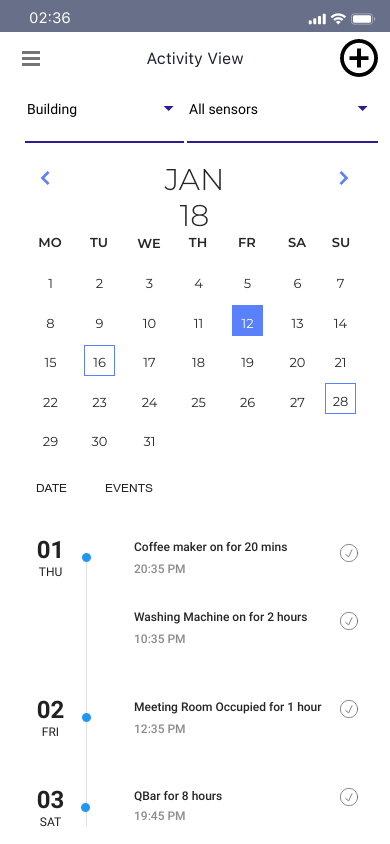
\includegraphics[width=0.59\linewidth]{./img/activityCalendar.png}
  \caption{ Activity Calendar of Building Management System.  }
  \label{fig:activityCalendar}
\end{figure}



\section{Experimental Evaluation}
\label{section:evaluation}
The IFC file used for input to the BIM parser is a 3 storied office building in Paris and consists nearly 120,000 IFC entries. There are 139 walls, 122 spaces, 139 walls, 89 doors, and 5 windows covering a net area of 3100 m$^2$.  


\begin{table}[]
\caption{Region of Interest Profiling}
\label{table:roiprofiling}
\centering
\begin{tabular}{|l|l|}
\hline
Space Name       & Seating Capacity \\ \hline
Sanitary     &  1    \\ \hline
Bathroom       & 1   \\ \hline
Electricity Room    & 0    \\ \hline
Meeting Room & 4   \\ \hline
Unused Room & 0 \\ \hline
Hardware Zone & 4   \\ \hline
Elevator & 4   \\ \hline
Private Office & 4 \\ \hline
Working Zone & 4 \\ \hline
Entrance & 1 \\ \hline
Kitchen & 12   \\ \hline
Reception & 2  \\ \hline
 {Passage}          &  {0}   \\ \hline
 {Environment}      &  {0}   \\ \hline
 {Marketing}        &  {10}  \\ \hline
 {Developers}       &  {16}   \\ \hline
\end{tabular}
\end{table}

\subsection{IFC Parsing}

 \begin{figure}[h]
\centering
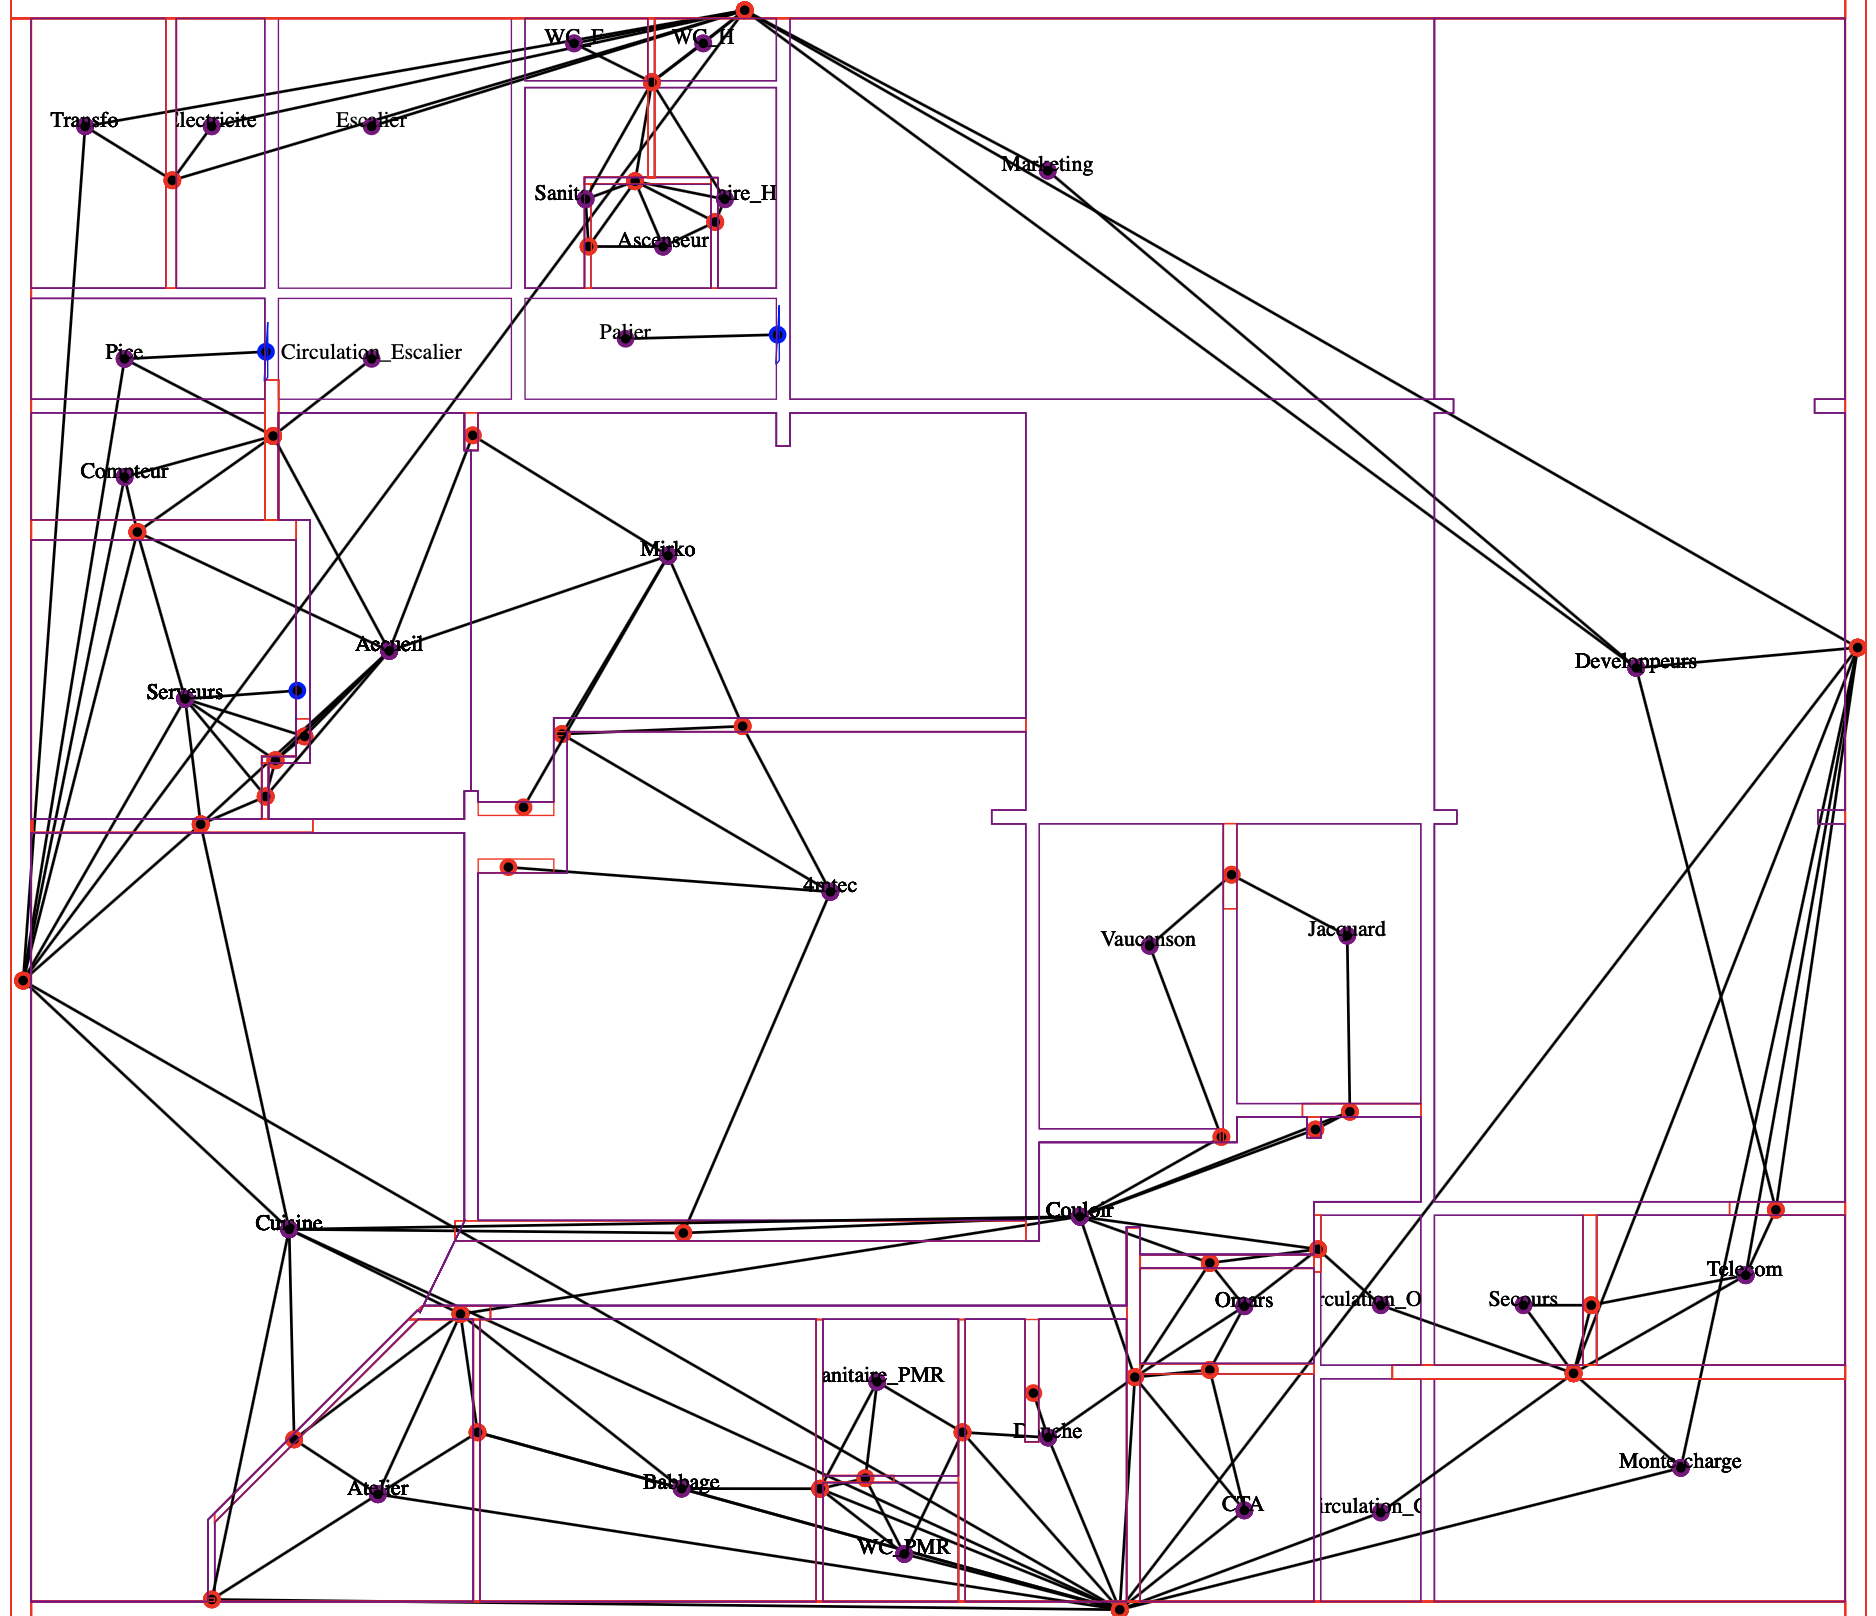
\includegraphics[width=.5\textwidth]{img/partial-graph.png}
\caption{Partial Graph formed by a slicing plane }
\label{fig:partial-graph}
\bigbreak
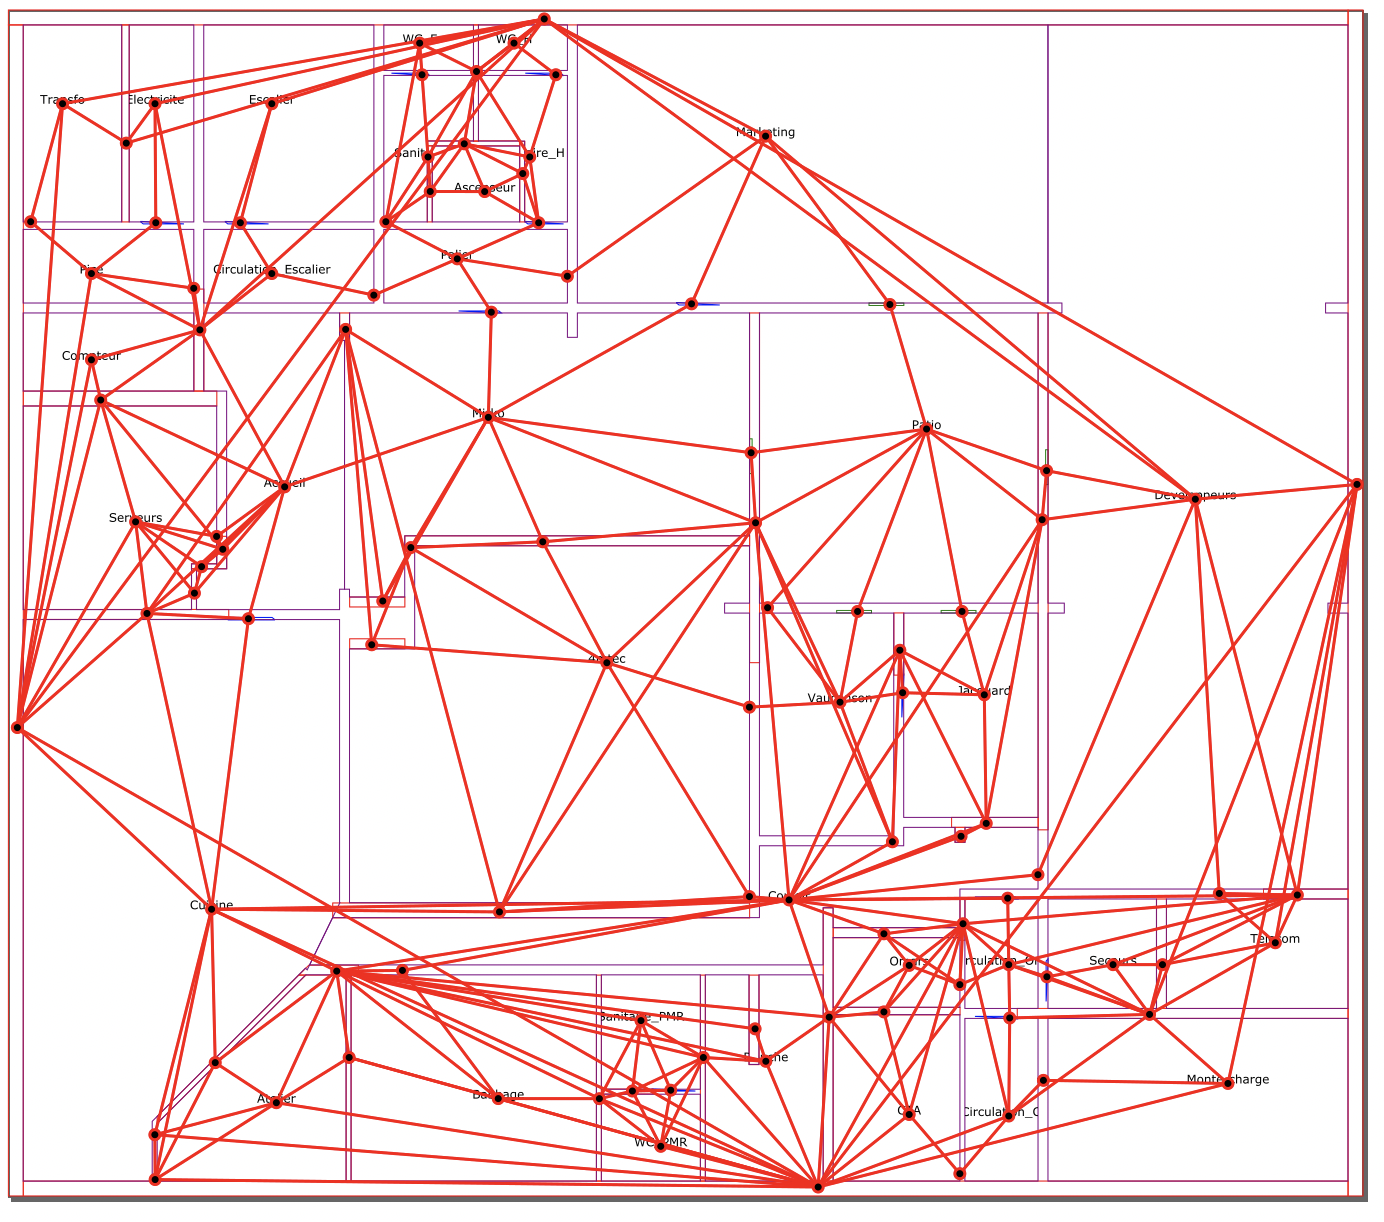
\includegraphics[width=.5\textwidth]{img/full-connectivity.png}
\caption{ Connectivity Graph obtained from Superimposing images}\label{fig:full-connectivity}
\end{figure}


Entire building is parsed by setting the direction of cutting plane along Z axis (0,0,1) and the slicing happens at every $\Delta h$ = 0.5 meter on interval $I_h = [-10, 10] $ resulting in a maximum of$\frac{I_h}{\Delta h} = 40 $ images per element.  The IFC storeys arranged from bottom to top are underground parking slot, basement, office floor and first floor. The spatial connectivity graph $G^S$ of the building, made of 340 nodes and 1159 links is derived by superimposing images of multiple elements per storey and inferring storey links. The partial graph $G^S$ formed by a single slicing plane $\Xi = (0,0,2.5)$ as shown in Figure \ref{fig:partial-graph} corresponds to a office floor-plan. The effect of combining multiple images yields a well connected graph of 16 spaces as shown in Figure \ref{fig:full-connectivity}. The space-space linkage ($G^P$) is made up of 16 nodes and 24 edges as shown in Figure \ref{fig:energygraph}. We add the seating capacity of the spaces in Table \ref{table:roiprofiling} and proceed next towards collecting ambient sensor data from 3 of the spaces to infer human-space interaction.



\subsection{Occupancy Prediction}

% \begin{figure}
% \centering
%   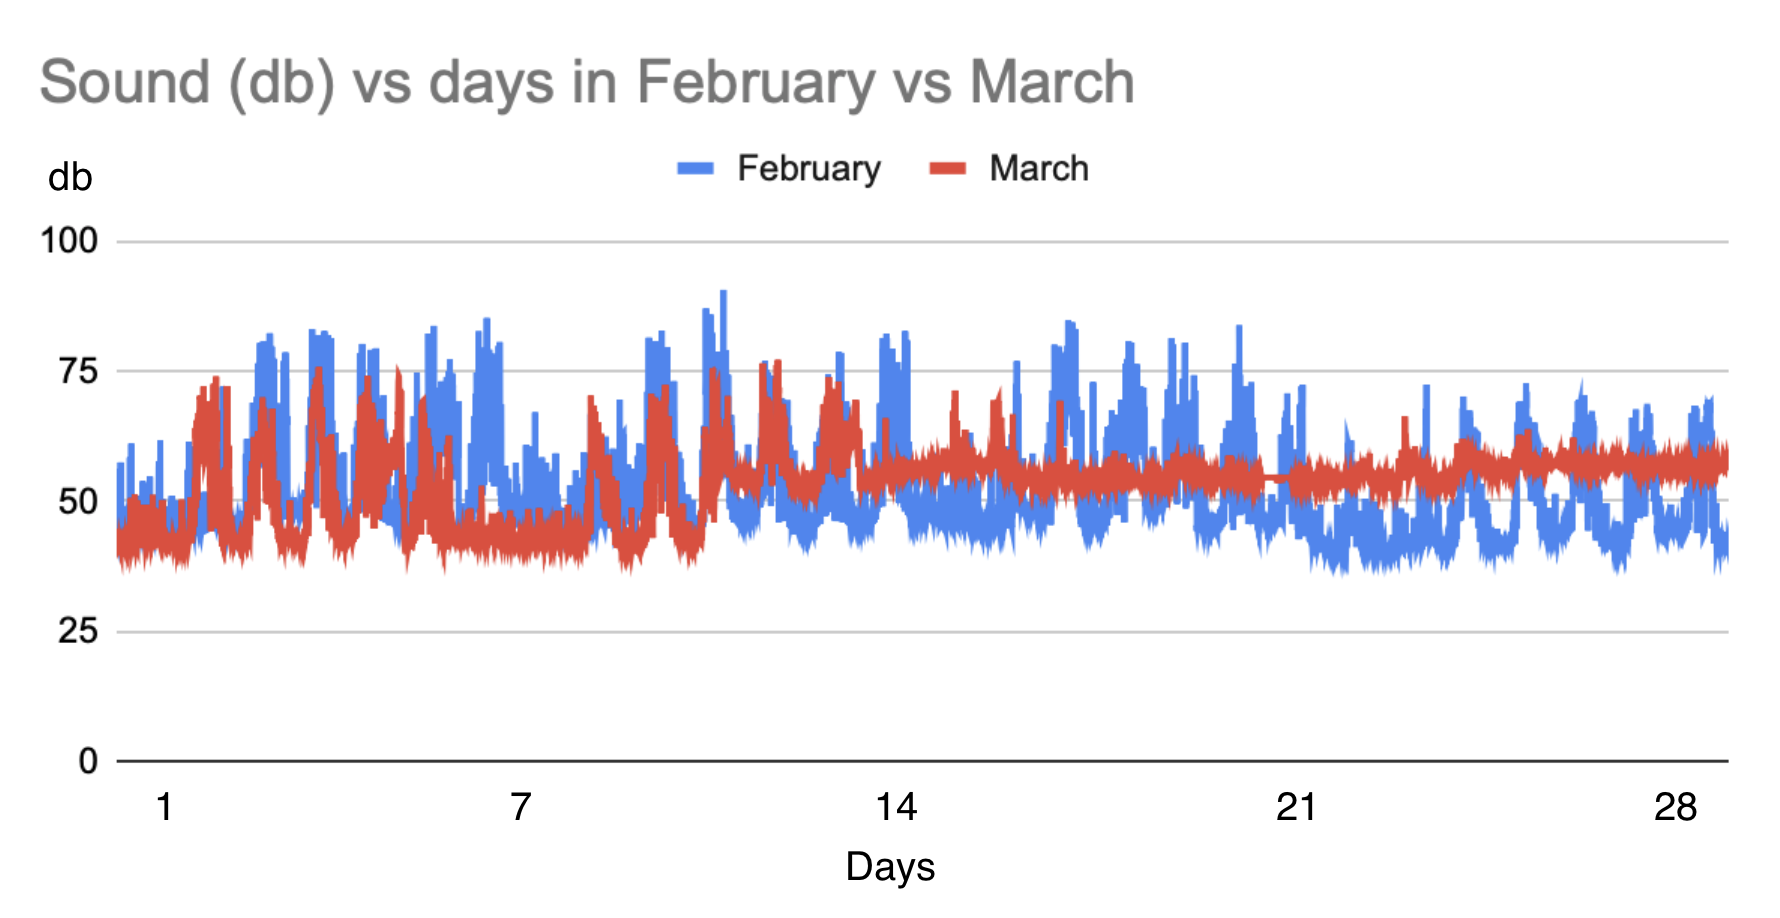
\includegraphics[width=1\linewidth]{./img/soundComparison.png}
%   \caption{ Sound Intensity (in decibels) variation 1 month before (blue) and after (in red) pandemic lockdown, 2020 }
%   \label{fig:soundComparison}
% \end{figure}



\begin{figure}
\centering
  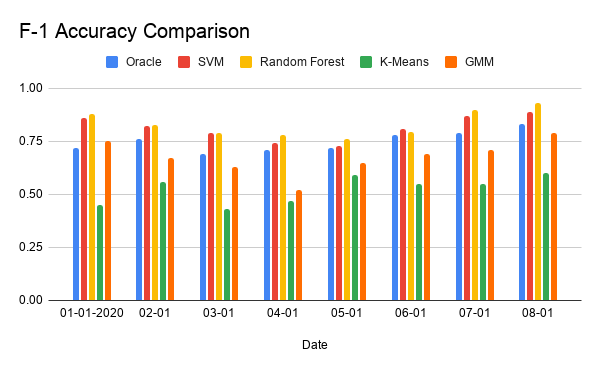
\includegraphics[width=1\linewidth]{./img/f1Accuracy.png}
  \caption{ Comparison between losses of oracle and trained models. }
  \label{fig:f1Accuracy}
\end{figure}


\begin{table}[]
\caption{Experimentally determined sensor weights used for activity discovery. }
\label{table:sensorweights}
\centering
\begin{tabular}{|l|l|}
\hline
Sensor      & Weight \\ \hline
CO$_2$      & 0.1    \\ \hline
Light       & 0.2    \\ \hline
Humidity    & 0.1    \\ \hline
Temperature & 0.1    \\ \hline
Sound       & 0.3    \\ \hline
Motion      & 0.2    \\ \hline
\end{tabular}
\end{table}

The test bed consists of 2.1 Million Sensor readings each sampled from 3 room: a kitchen, private space and a meeting room . The sensor channels are luminous intensity(lux), sound (decibel), temperature (celcuis), relative humidity, motion, energy meter (milliWattHour). 
%The data represents pre-pandemic and post pandemic office building usages. 
% For example, Figure \ref{fig:soundComparison} shows the sound distributions of February and March plotted against day of month on X axis in blue and red respectively. Notice that the red line falls around week starting from 14th March,2020 which coincides with lock-down issued in France for the first time. The distinct pattern of 5 broad and 2 small spikes corresponding to 5 working and 2 weekend days as per regular calendar.  

The first step towards activity detection is automated data labelling, which is done by varying the time dilation parameter $\tau$ between 1 to 5, representing a resolution of 5 to 30 minutes. We observe the most optimal detection with $\tau = 2$ or a 10 minute comparison window. The weight table for the sensors are based on the entropy distribution as shown in Table \ref{table:sensorweights}. The labelled data is up-sampled to reduce class imbalance via Synthetic Minority Oversampling Technique \cite{chawla2002smote}. Next comes training supervised learning models namely XgBoost, Support Vector Machine and Decision Trees on the auto-labelled data via a k-fold cross validation (k=5). We compare the models via the performance metric of F-1 Score which is the harmonic mean of precision and recall. The supervised learners have a mean F1 score of 0.81-0.85 with a variance of 0.01- 0.06. The baseline comparison in our setting are unsupervised models. For each class we averaged the input feature set into a single dimension vector to initialize the seed for K-Means and Gaussian Mixture Model (GMM). GMM performed slightly better than K-Means although the averaged F1 score varied between 0.65-0.75 with a variance of 0.07-0.1. Mean F-1 score is shown in Fig \ref{fig:f1Accuracy} and refers to the monthly model performance with retraining on previous month's data. We observe that efficiency of SVM and Random Forest is higher than the oracle by 9 to 16 $\%$ while unsupervised models fail to capture intuitive heuristics embedded in the oracles. We cross validate our observations by taking the cosine distance between cluster-centers, a averaged input data vector per class predicted by each classifier. The cosine distance between cluster-centers of supervised and unsupervised model groups is 0.19 while intra-group difference between K-Means and GMM is 0.27  The maximum distance of cluster-centers between SVM, XGboost and Random Forest came out as 0.07. Additionally we cross check by filtering through sanity checks of no occupancy on weekends, holidays and at night.
%The execution stats for 8 months with bi-monthly update policy on 3 rooms each with 2 activities consists of training approximately $8 \times 3 \times 4 = 96$ models with a 40-60 $\%$ discard-drop off rate. 

\begin{figure}
\centering
  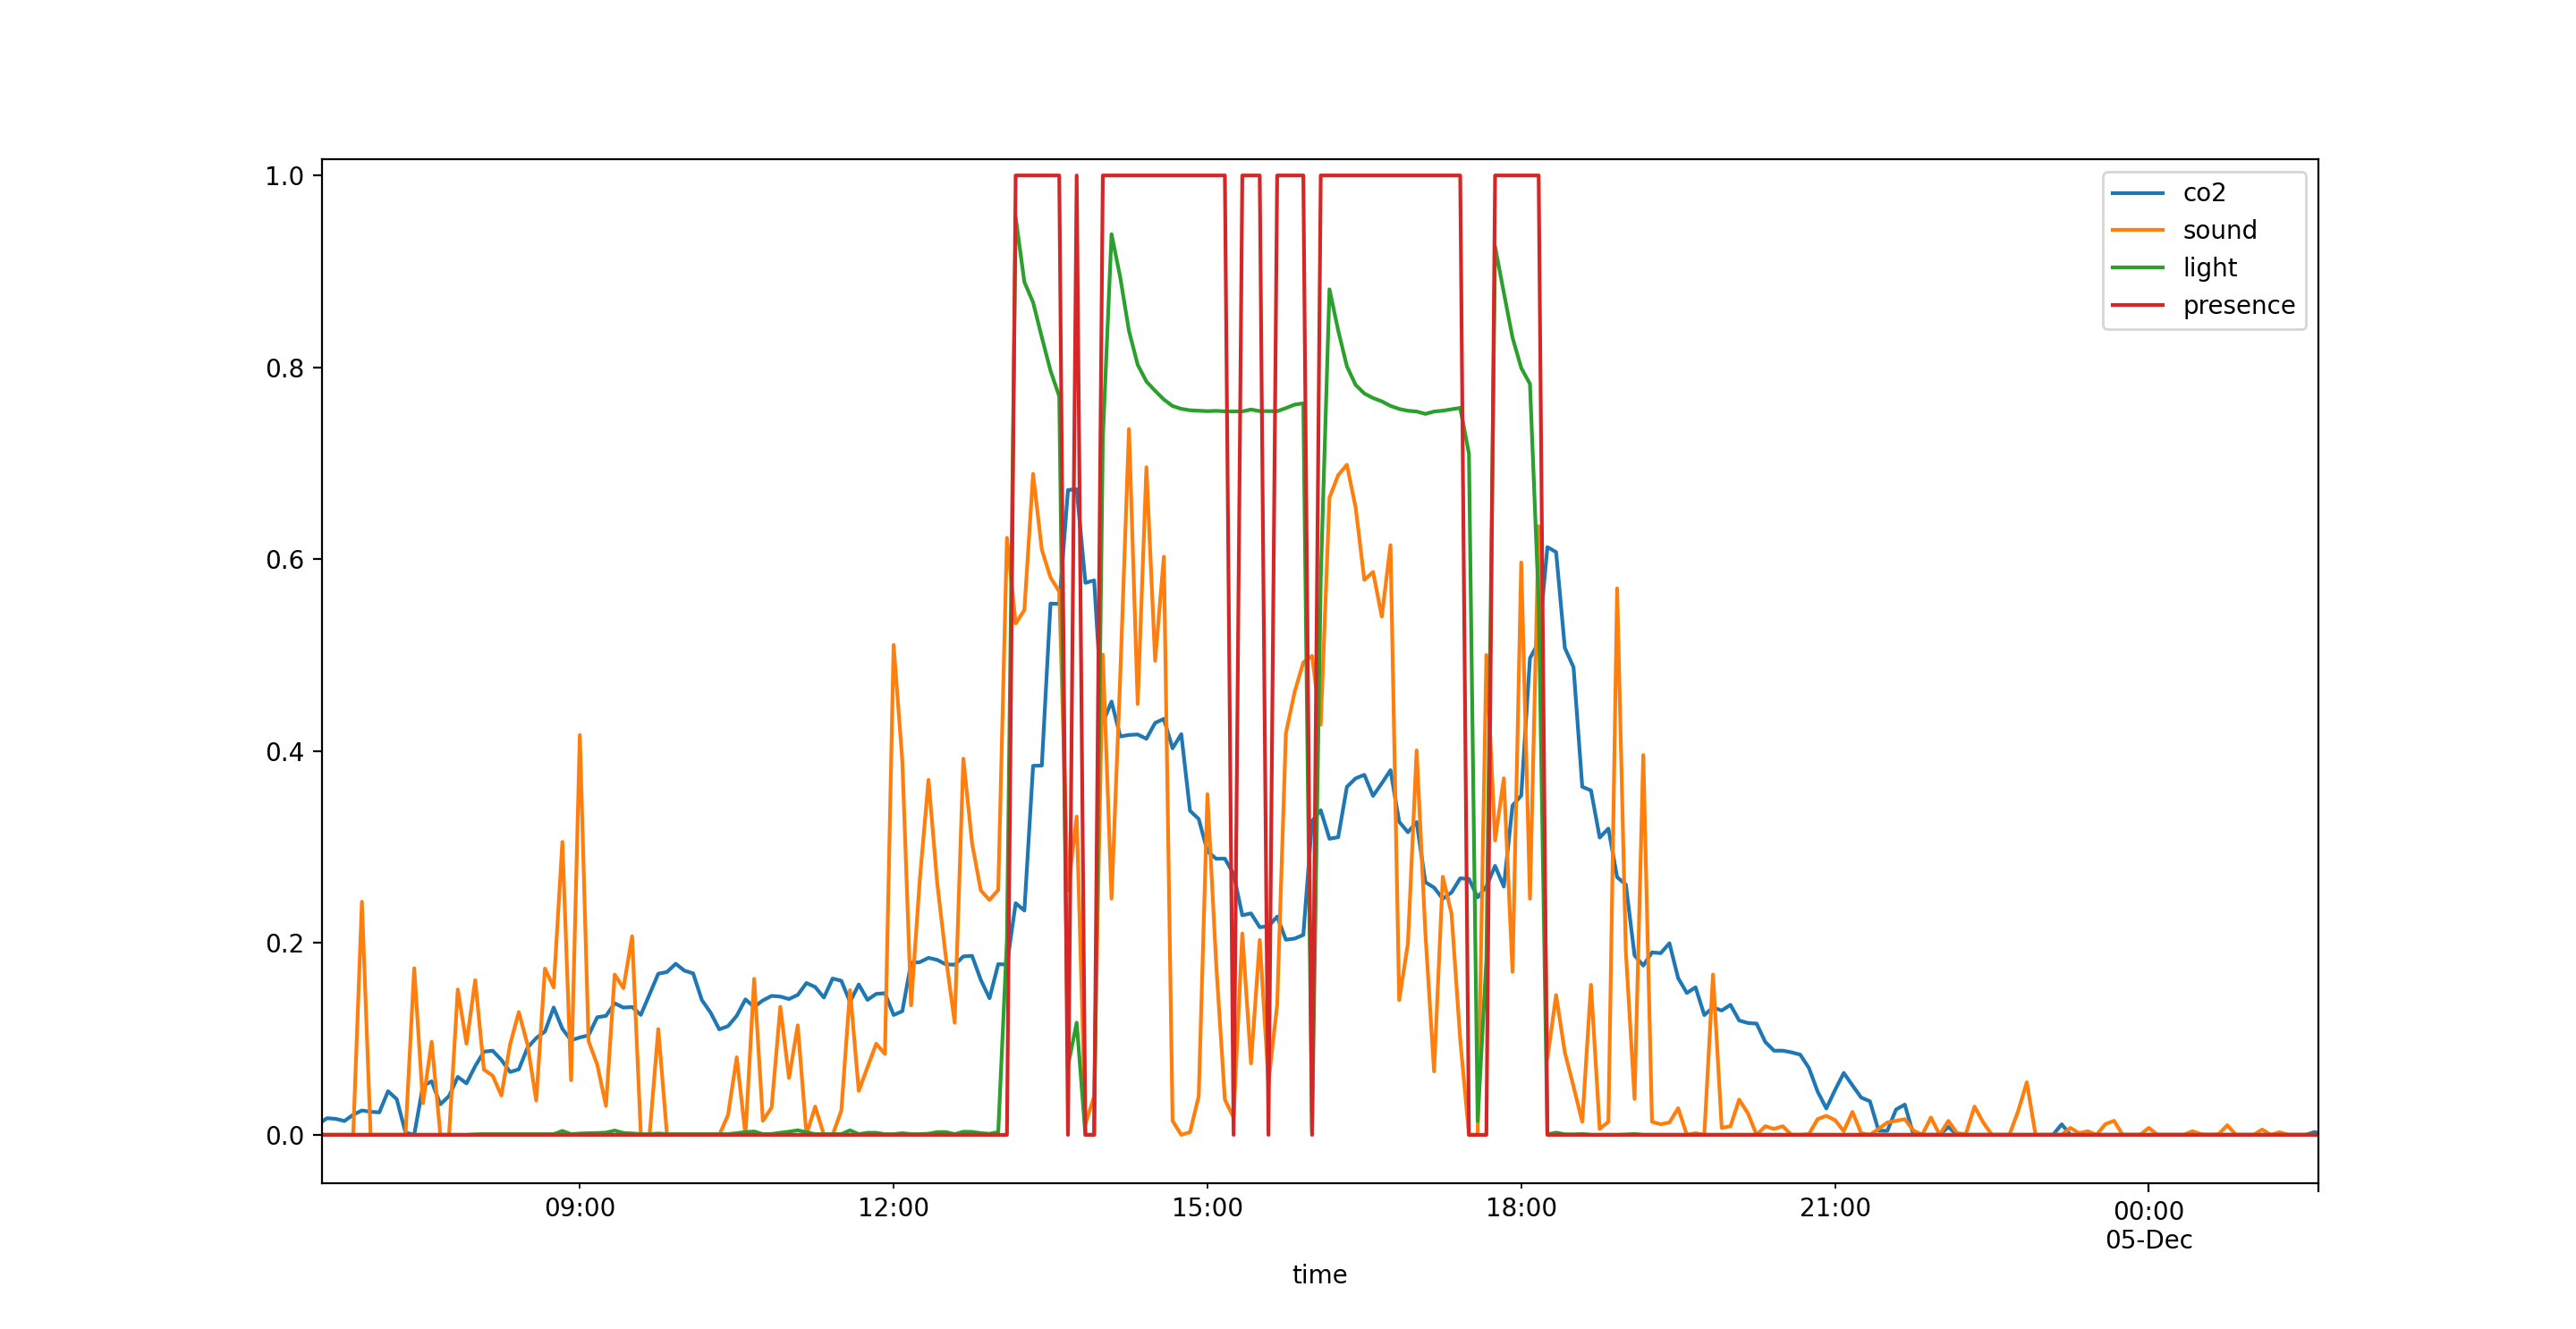
\includegraphics[width=1\linewidth]{./img/occupancy.png}
  \caption{ Sensor values and detected occupancy on a 0-1 scale normalized view.}
  \label{fig:occupancy}
\end{figure}


\subsection{Energy Insights}


 \begin{figure}[h]
\centering
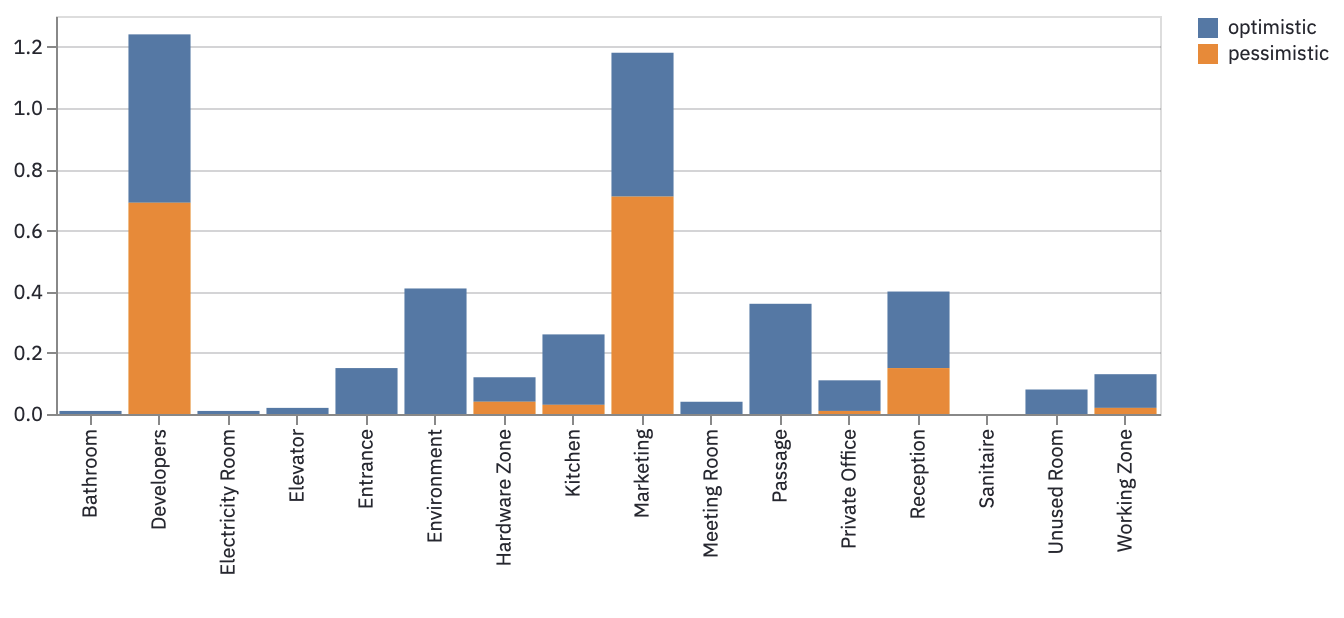
\includegraphics[width=.5\textwidth]{img/full-occupancy.png}
\caption{Energy Score Distribution of spaces assuming fully occupancy }\label{fig:full-occupancy}
\bigbreak
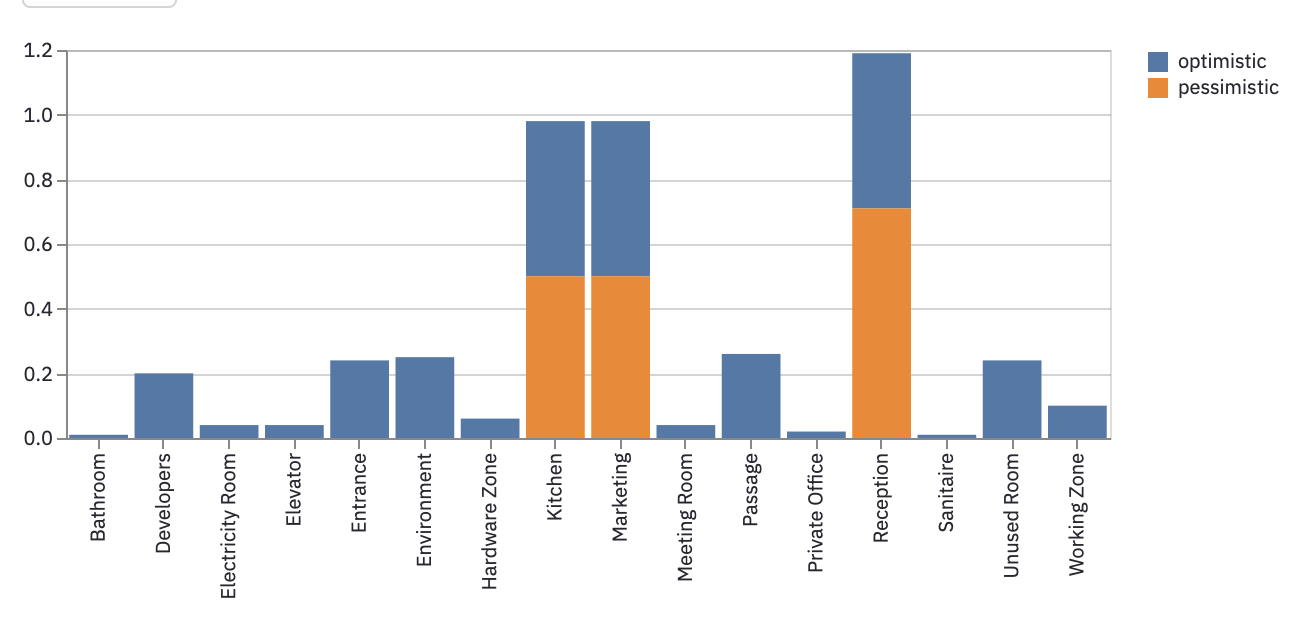
\includegraphics[width=.5\textwidth]{img/partial-occupancy.png}
\caption{Lunch time office occupancy scenario with dynamic edge weights}\label{fig:partial-occupancy}
\end{figure}

%  \begin{figure}[h]
% \centering
% 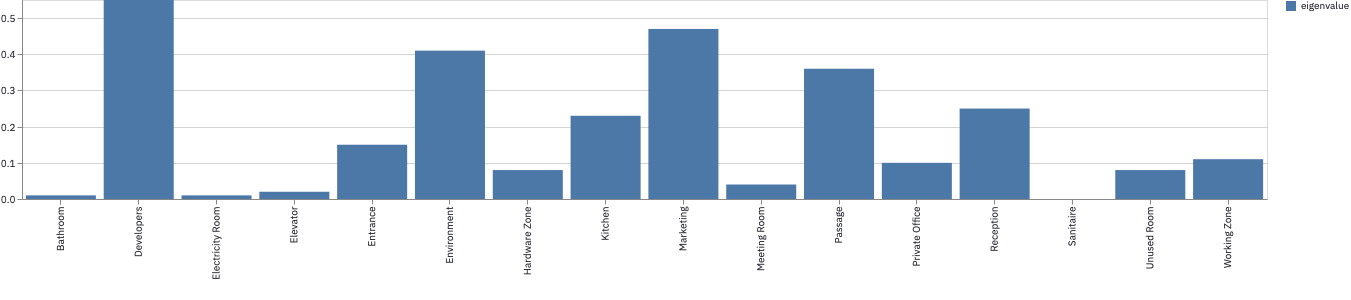
\includegraphics[width=.5\textwidth]{img/optimistic-fulloccupancy.png}
% \caption{Optimistic Mixing}\label{fig:optimistic-fulloccupancy}
% \bigbreak
% 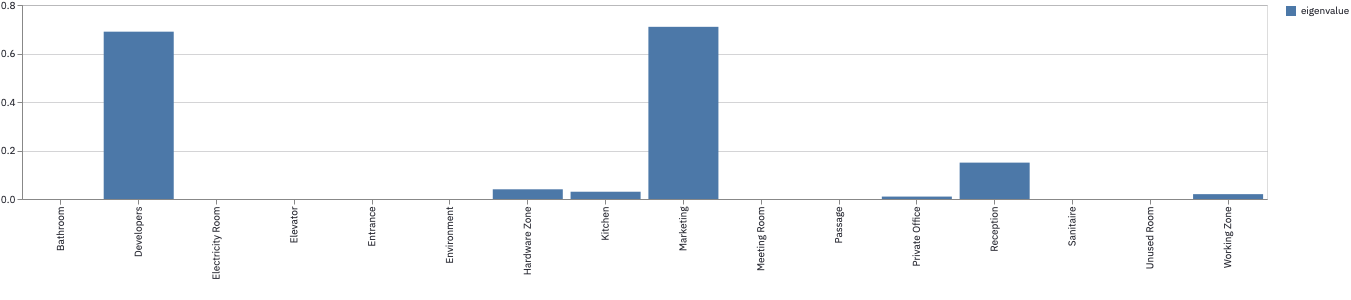
\includegraphics[width=.5\textwidth]{img/pessimistic-fulloccupancy.png}
% \caption{Pessimistic Mixing}\label{fig:pessimistic-fulloccupancy}
% \end{figure}

Now, the system leverages the semantic usage of a space to generate energy insights. For example, in the case of full occupancy $O^t=[1]_{1\times I}$ represented by a vector of all ones, the ratio of eigenvalues gives an intuition about spatial disintegration of electrical power. Figure \ref{fig:full-occupancy} shows the belief distribution against pessimistic and optimistic dispersion along edges of the fully occupied floor-plan as denoted by Equation \ref{eq:maxdispersion}. The 3 highest score sums correspond to  the Developer's Zone (1.25), Marketing Zone (1.11) and Reception (0.4). While first 2 spaces can be explained in term's of seating capacity, the importance of reception reflects the likelihood of space-usage for entering or exiting the floor-plan. The passage has a score of 0 under minimal mixing strategy, indicating if adjacent activities are concentrated in their respective zones, then the passage is least likely to be used. But it becomes the fourth most important space (0.36) when occupants are shuffling spaces and is explainable by high degree centrality. The edge weight formulation helps to answer questions like "If there are no people at the developer's floor, hardware zone and office what are the most likely occupied places?". Figure \ref{fig:partial-occupancy} helps to answer the question by showing the top 3 spaces as the reception (1.05), marketing zone (0.97) and kitchen (0.96). This scenario corresponds to the spatial distribution of people during lunch time and the output is affirmed by the regular ground truth. 




%  A 24 hour day is divided into 96 intervals of 15 minutes each and for every interval and for each interval Algorithm \ref{algo:energyOracle} assigns a score to a space accordingly to its  utility value. The motivation behind the work is to identify which spaces are useful and where power connection is most likely to be shut down.
 
%  From the spatial graph, we extract paths with either the source or sink node having ambient sensors. Now from the temporal usage we derive a historical occupancy distribution in sensor enabled spaces. 


% \begin{algorithm}[]
% \SetAlgoLined
% \KwResult{ Load Space Shutdown  (LSS, t) } 
%  LSS = $\{v | O(v, t ) = 0\} $   $\forall v \in G(V, E) $ \;
%  OccupiedSpaces (OS) =  $\{v | O(v, t ) =   1\} $   $\forall v \in G(V, E) $ \;
%  UnknownSpaces (US) = V - LSS - OS \;
%  BeliefUnknownSpace (BUS)  = \{ u : 0 \} $\forall u \in$ US  \;
%  \For{$\forall$ (u,v) $|$ u $\in$ OS, v $\in$ US}{
%  NodeList = Path(u,v) \;
%  \For{node $\in$ NodeList}{
%  BUS[node] += Apriori(node) \;
% }
%  }
%   return $LSS$\;
%  \caption{Load Space Shutdown }
%  \label{algo:energyOracle}
% \end{algorithm}





\section{Conclusion}
\label{section:conclusion}

The work introduces the blueprint for a generic building management system that auto acquires ambient intelligence and translates into energy insights. The IFC parsing technique has been pivotal in understanding buildings as a dynamic graph structure.
We present a simple model of human-space interaction which can reinforce the temporal dynamics in real-time. We show that it is indeed feasible to embedded heuristics as oracles and then train statistical models for better prediction accuracy.
Future work lies in a theoretical study of oracles with analysis of worse case bounds and convergence guarantees and addition of electrical consumption data readings. In a nutshell, the work contributes towards an open-source smart building management system which showcases the possibility of business intelligence with an ad-hoc non intrusive IoT integration.
%Since the data processing is event specific, a major advantage is in fast adoption for a new label or target and triggering dependent learners to revise and retrain if necessary. 


\section{Acknowledgements }
This work has been partially supported by the Multi-disciplinary Institute on Artificial Intelligence MIAI at Grenoble Alpes (ANR-19-P3IA-0003) and GRECO project (Resource manager for cloud of things) funded under the reference ANR-16- CE25-0016. Angan Mitra is supported by the convention CIFRE at ANRT 2018/0874.
% The sample data used for experimental analysis for 8 months is at  https://github.com/AnganMitra/SmartBuildingDATA.


\bibliographystyle{IEEEtran}
\bibliography{ref.bib}

\end{document}

% The test-bed collected ubiquitously from open office, meeting room and kitchen consists of 1.4 Million sensor data readings, sampled at every 5 minutes leading to 288 samples a day, totalling to 208K samples in 8 months. Each data point contains temperature (in Celcius), relative humidity, noise levels (in decibels), power (in Watts), luminous intensity (in lux) and indoor air quality (in ppm) readings.


% \begin{figure}
% \centering
%   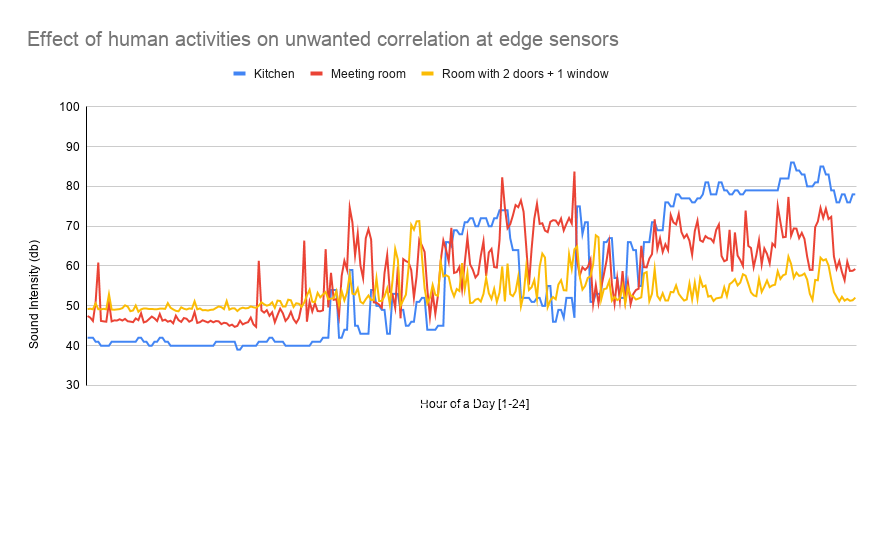
\includegraphics[width=1\linewidth]{./img/activityCorrelation.png}
%   \caption{ Varying acoustic intensity between 3 spaces on the same floor within a single office space on a day. Note the rise in sound levels at other rooms when a party takes place from 18:00 hours at the kitchen (in blue) although people desert working spaces (in red and yellow). }
%   \label{fig:activityCorrelation}
% \end{figure}


% A smart building data can reflect some interesting observations for example Fig. \ref{fig:activityCorrelation} exemplifies the effect of partying in a room causing a rise in sound detection at edge devices placed in other rooms. Sensor values can also be influenced by spatial factors such as absence or quantity or orientation of windows and doors. 
